\begin{figure}[p]
\lstset{frame=single}
\begin{center}
\begin{tabular}{@{}c@{\hspace{0.07\textwidth}}c@{}}
\begin{minipage}{0.42\textwidth}
\begin{lstlisting}[title={Old version code}]
public class LinkedList {
  class Node {
    Node next;
    int data;
  }
  private Node head;
}
\end{lstlisting}
\end{minipage} &
\begin{minipage}{0.42\textwidth}
\begin{lstlisting}[title={New version code}]
public class LinkedList {
  class Node {
    Node prev;
    Node next;
    int data;
  }
  private Node head;
  private Node tail;
}
\end{lstlisting}
\end{minipage}
\end{tabular} \\[2ex]
\begin{minipage}{0.9\textwidth}
\begin{lstlisting}[frame=single,title={Stub classes for the old version}]
public class r0_LinkedList {
  public LinkedList.Node head;
  public class Node {
    public LinkedList.Node next;
    public int data;
  }
}
\end{lstlisting}
\end{minipage} \\[2ex]
\begin{minipage}{0.9\textwidth}
\begin{lstlisting}[frame=single,title={Default \UPT-generated transformer}]
public class JvolveTransformers {
  public static void jvolveObject(
      LinkedList.Node to, r0_LinkedList.Node from) {
    to.prev = null; // no such field in from
    to.next = from.next;
    to.data = from.data;
  }
  public static void jvolveClass(LinkedList.Node unused) {}
  public static void jvolveObject(
      LinkedList to, r0_LinkedList from) {
    to.head = from.head;
    to.tail = null; // no such field in from
  }
  public static void jvolveClass(LinkedList unused) {}
}
\end{lstlisting}
\end{minipage}
\end{center} 
\vspace*{-2ex}
% 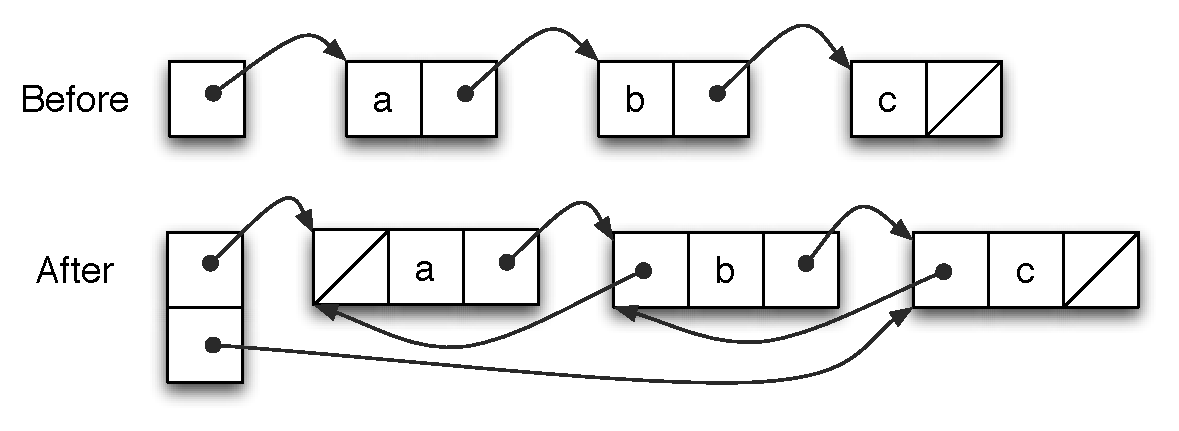
\includegraphics[scale=0.7]{100-images/linked-lists-without-gc}
\caption{An update that goes from a singly-linked to a doubly-linked list
\label{fig:singly-doubly}}
\lstset{frame=none}
\end{figure}
